101. $\cfrac{x^3-8x^2+15x}{x-3}\leqslant0\Leftrightarrow \cfrac{x(x^2-8x+15)}{x-3}\leqslant0\Leftrightarrow\cfrac{x(x-3)(x-5)}{x-3}\leqslant0.$ Применив метод интервалов, найдём ответ: $x\in[0;3)\cup(3;5].$
\begin{figure}[ht!]
\center{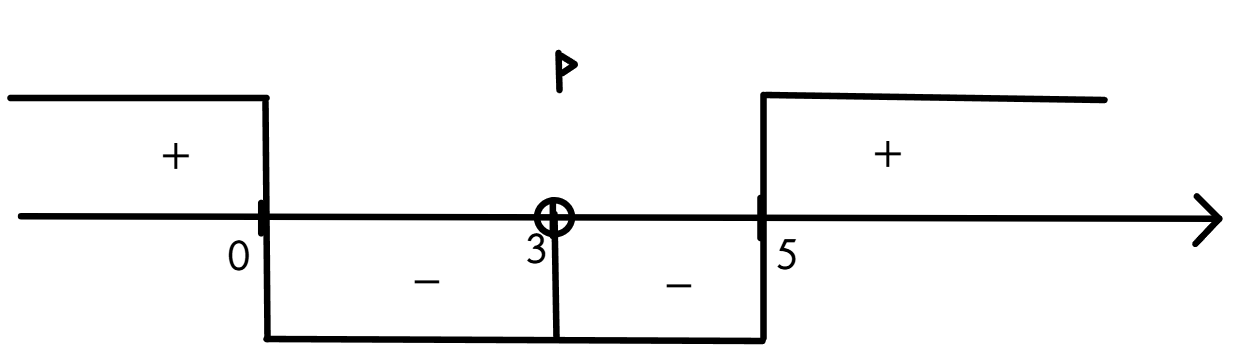
\includegraphics[scale=0.35]{int84.png}}
\end{figure}

ewpage
